\renewcommand{\arraystretch}{1.5}
\begin{tabular}{p{7cm}|p{4.5cm}|p{5cm}}
	\hline
	&
	\begin{minipage}{4cm}
		\textbf{\textit{Seriell}} 
	\end{minipage} & 
	\begin{minipage}{4.5cm}
		\textbf{\textit{Parallel}} 
	\end{minipage} \\
	Kompensation mit C &
    	\begin{minipage}{4cm}
    		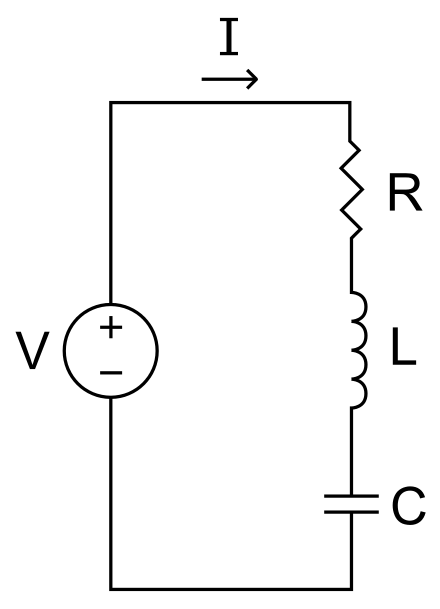
\includegraphics[height=3.5cm]{bilder/RLC-Seriell.png} \newline
        \end{minipage} & 
		\begin{minipage}{4.5cm}
			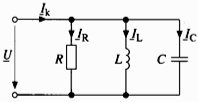
\includegraphics[width=3.5cm]{bilder/Parallelkompensation.png} \newline
		\end{minipage} \\
	Blindleistung &
		\begin{minipage}{4.5cm}
			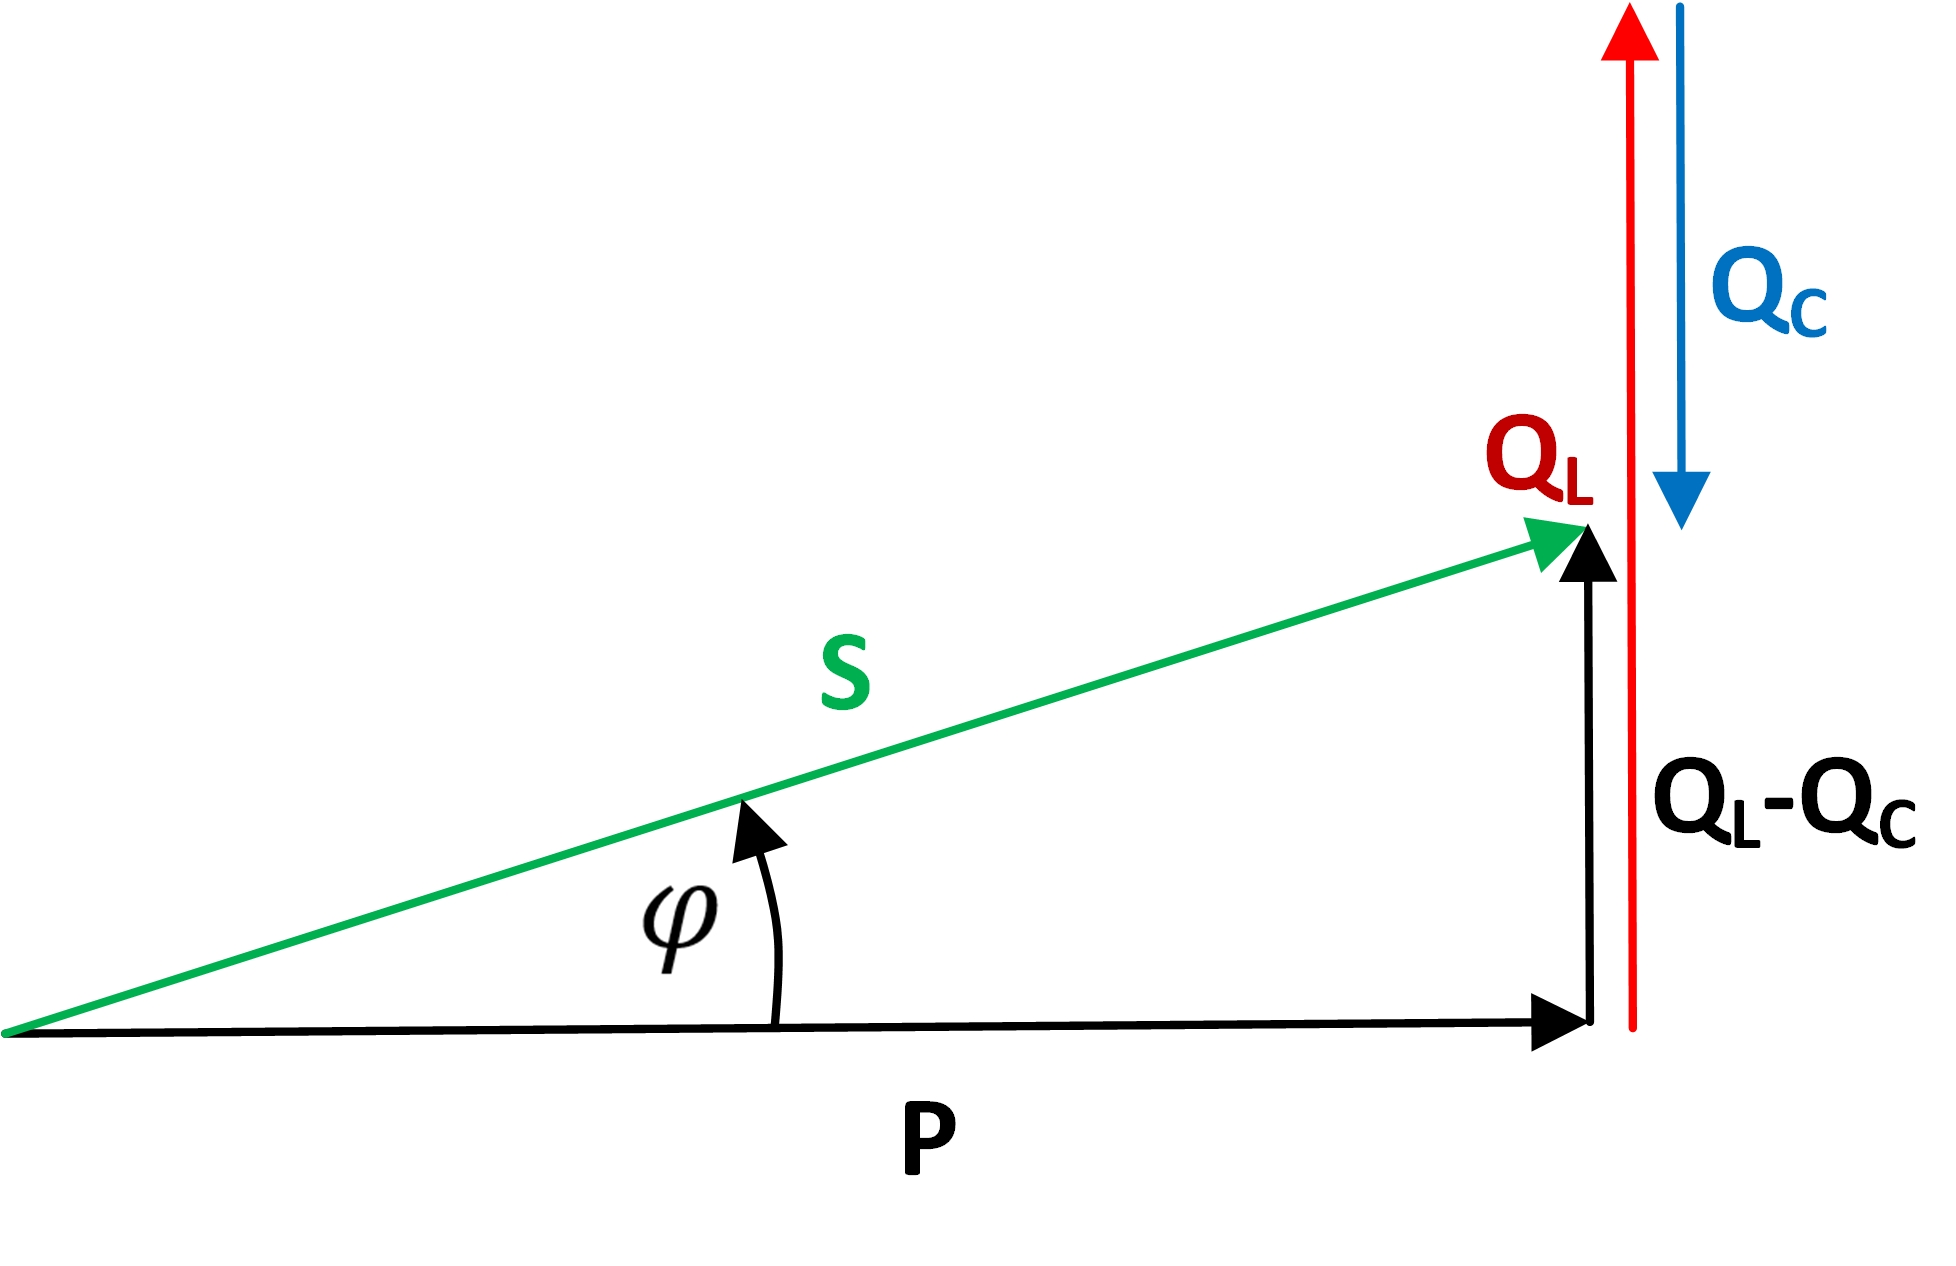
\includegraphics[width=3.5cm]{bilder/Blindleistungskompensation_RostBau.jpg} \newline
        \end{minipage} &
		\begin{minipage}{4.5cm}
        	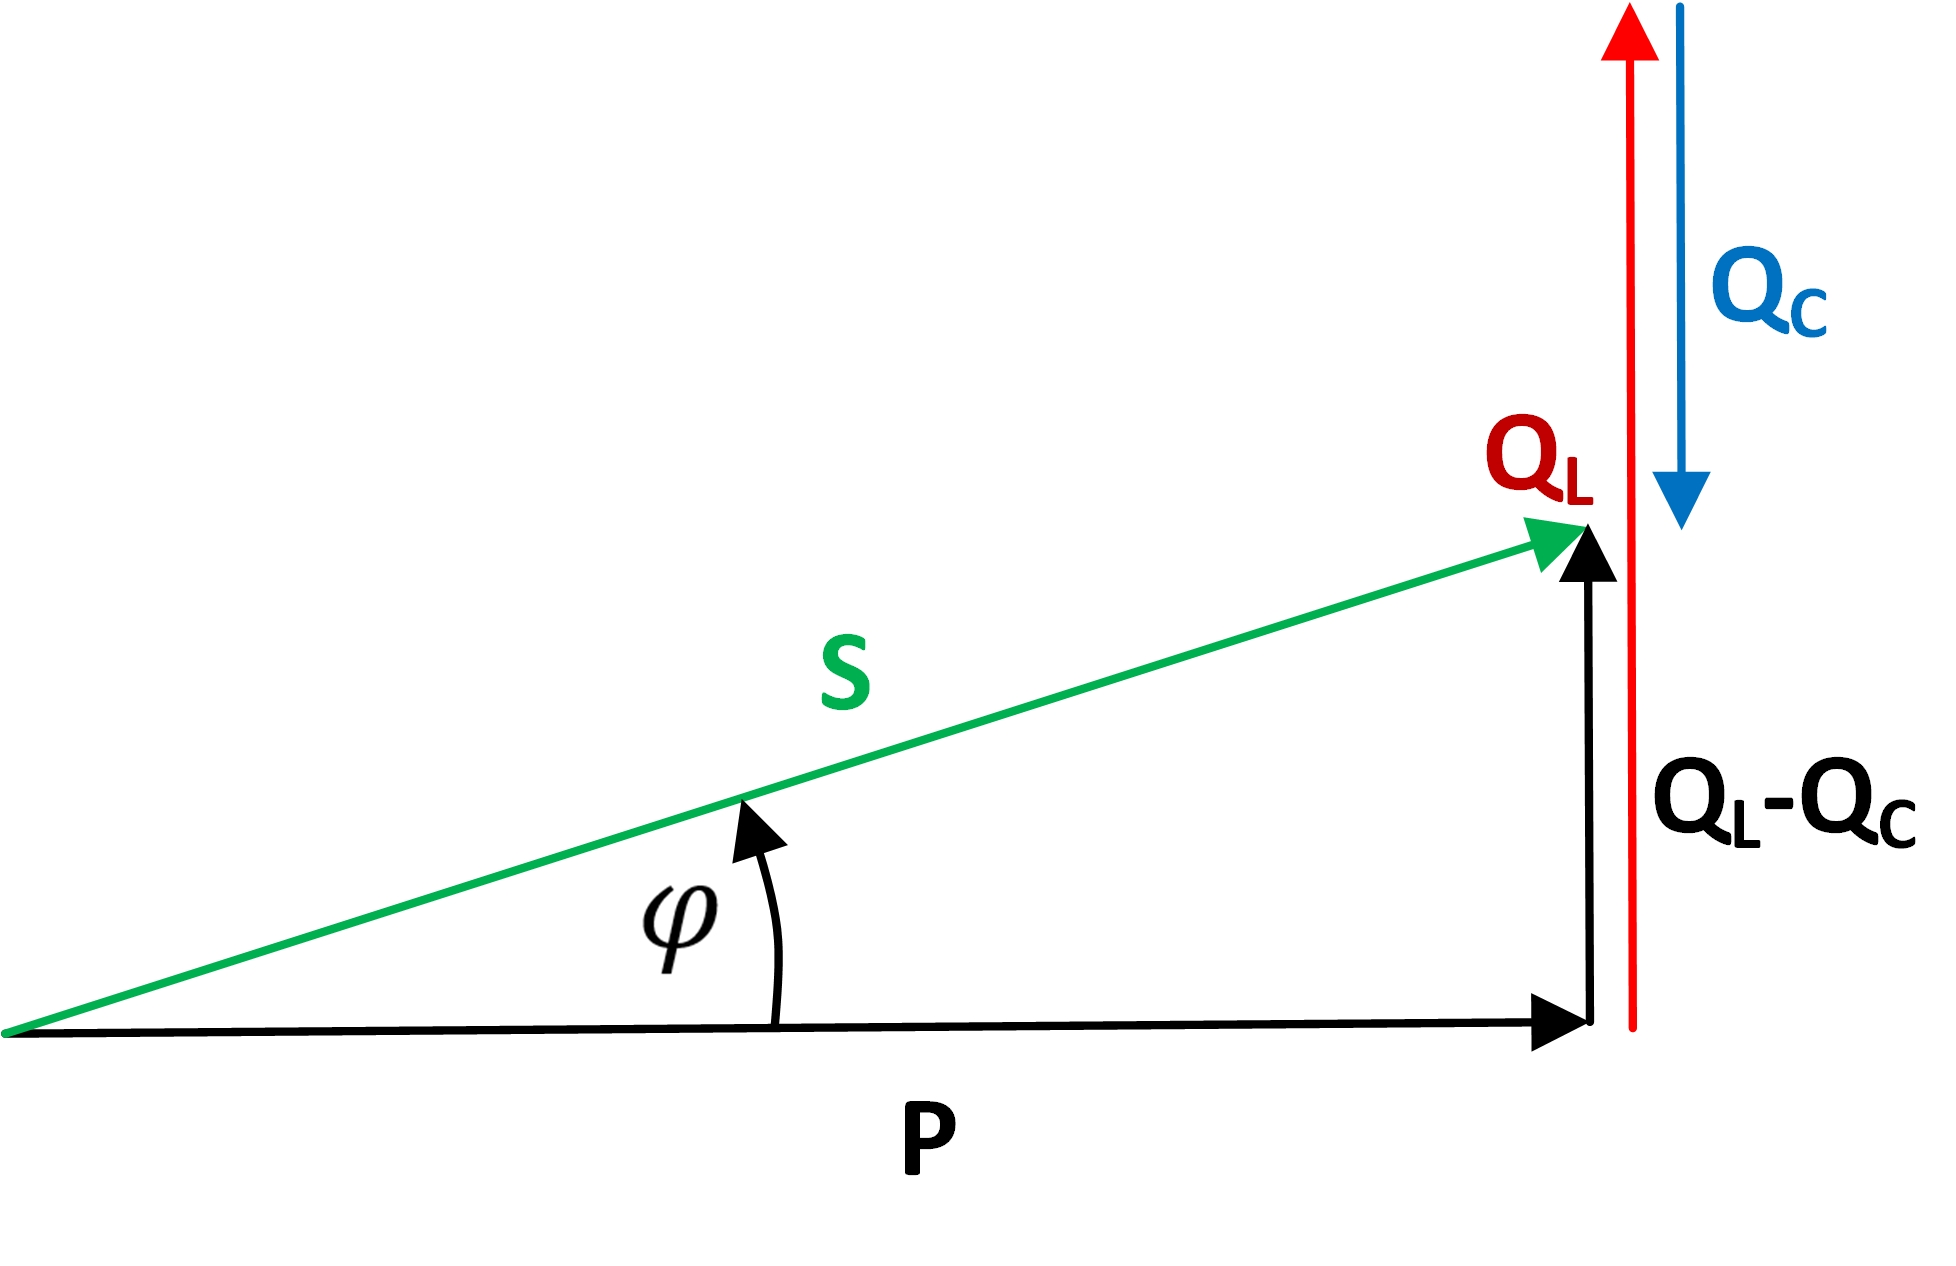
\includegraphics[width=3.5cm]{bilder/Blindleistungskompensation_RostBau.jpg} \newline
        \end{minipage} \\
	Spannungs/Strom -Verhältnisse &
		\begin{minipage}{4.5cm}
			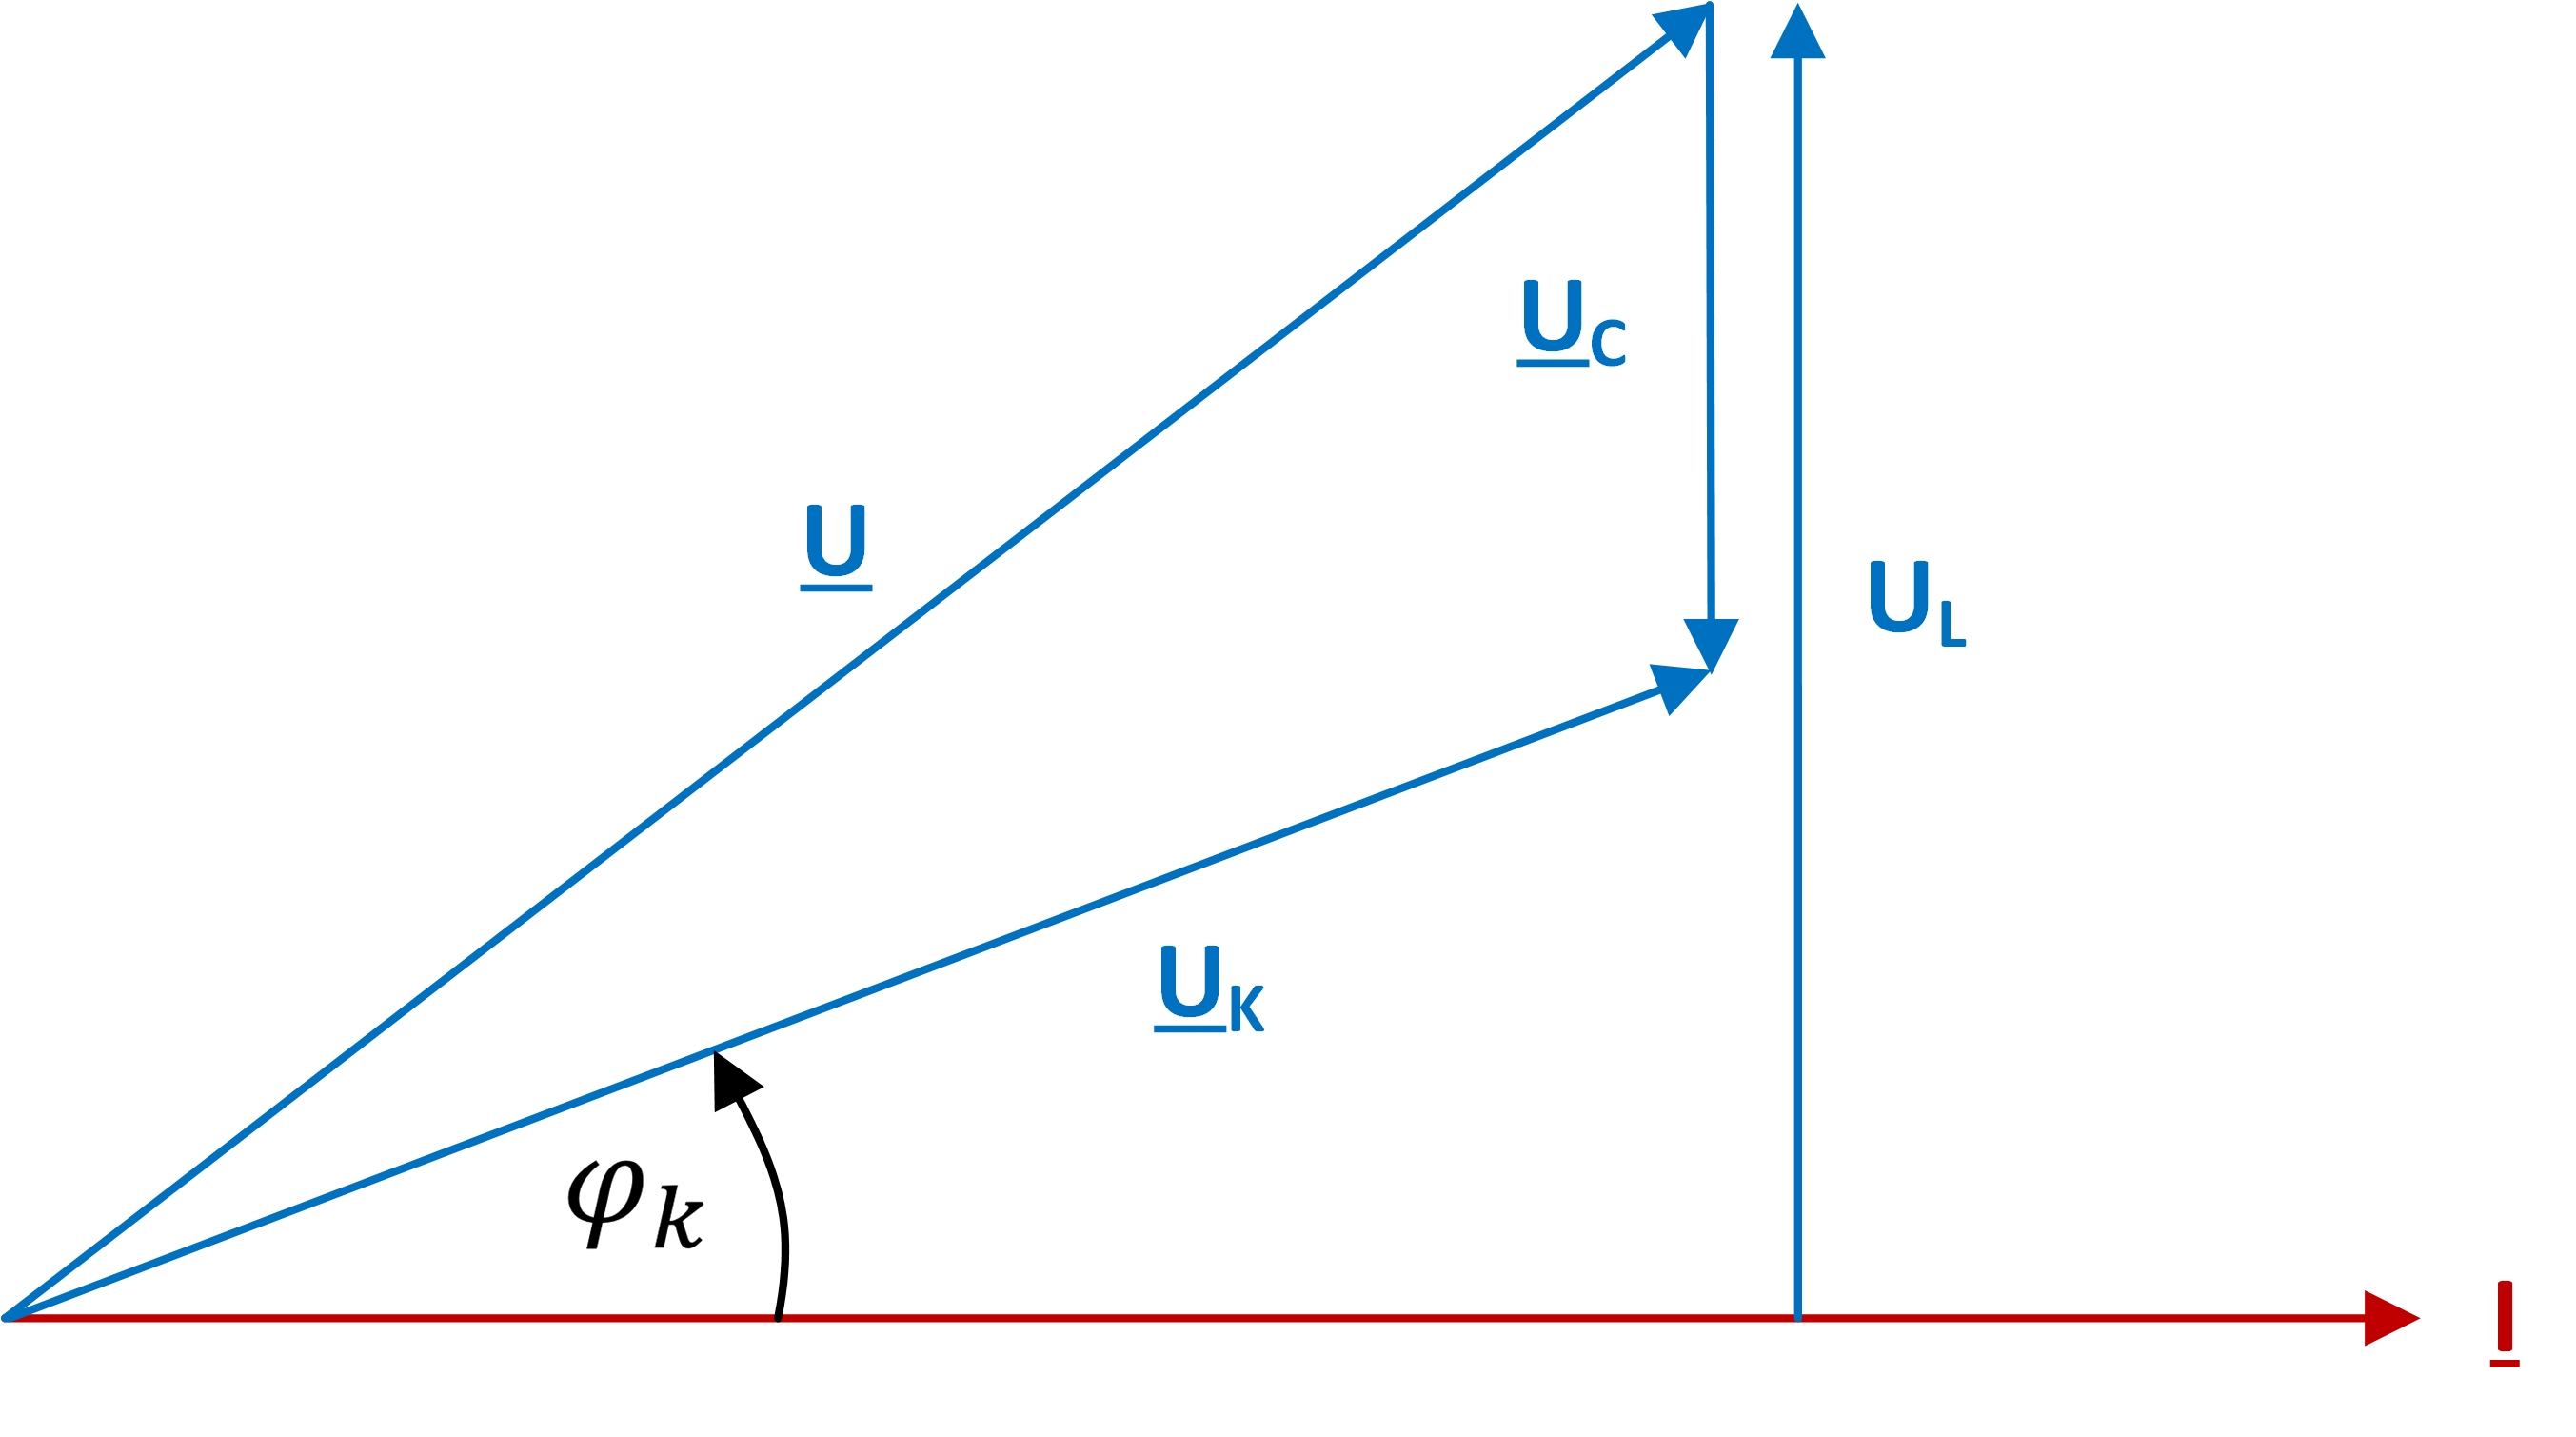
\includegraphics[width=3.5cm]{bilder/Seriell-Kompensation_RostBau.jpg}%%Blindstromkompensation.png%} \newline
		\end{minipage} &
		\begin{minipage}{4.5cm}
			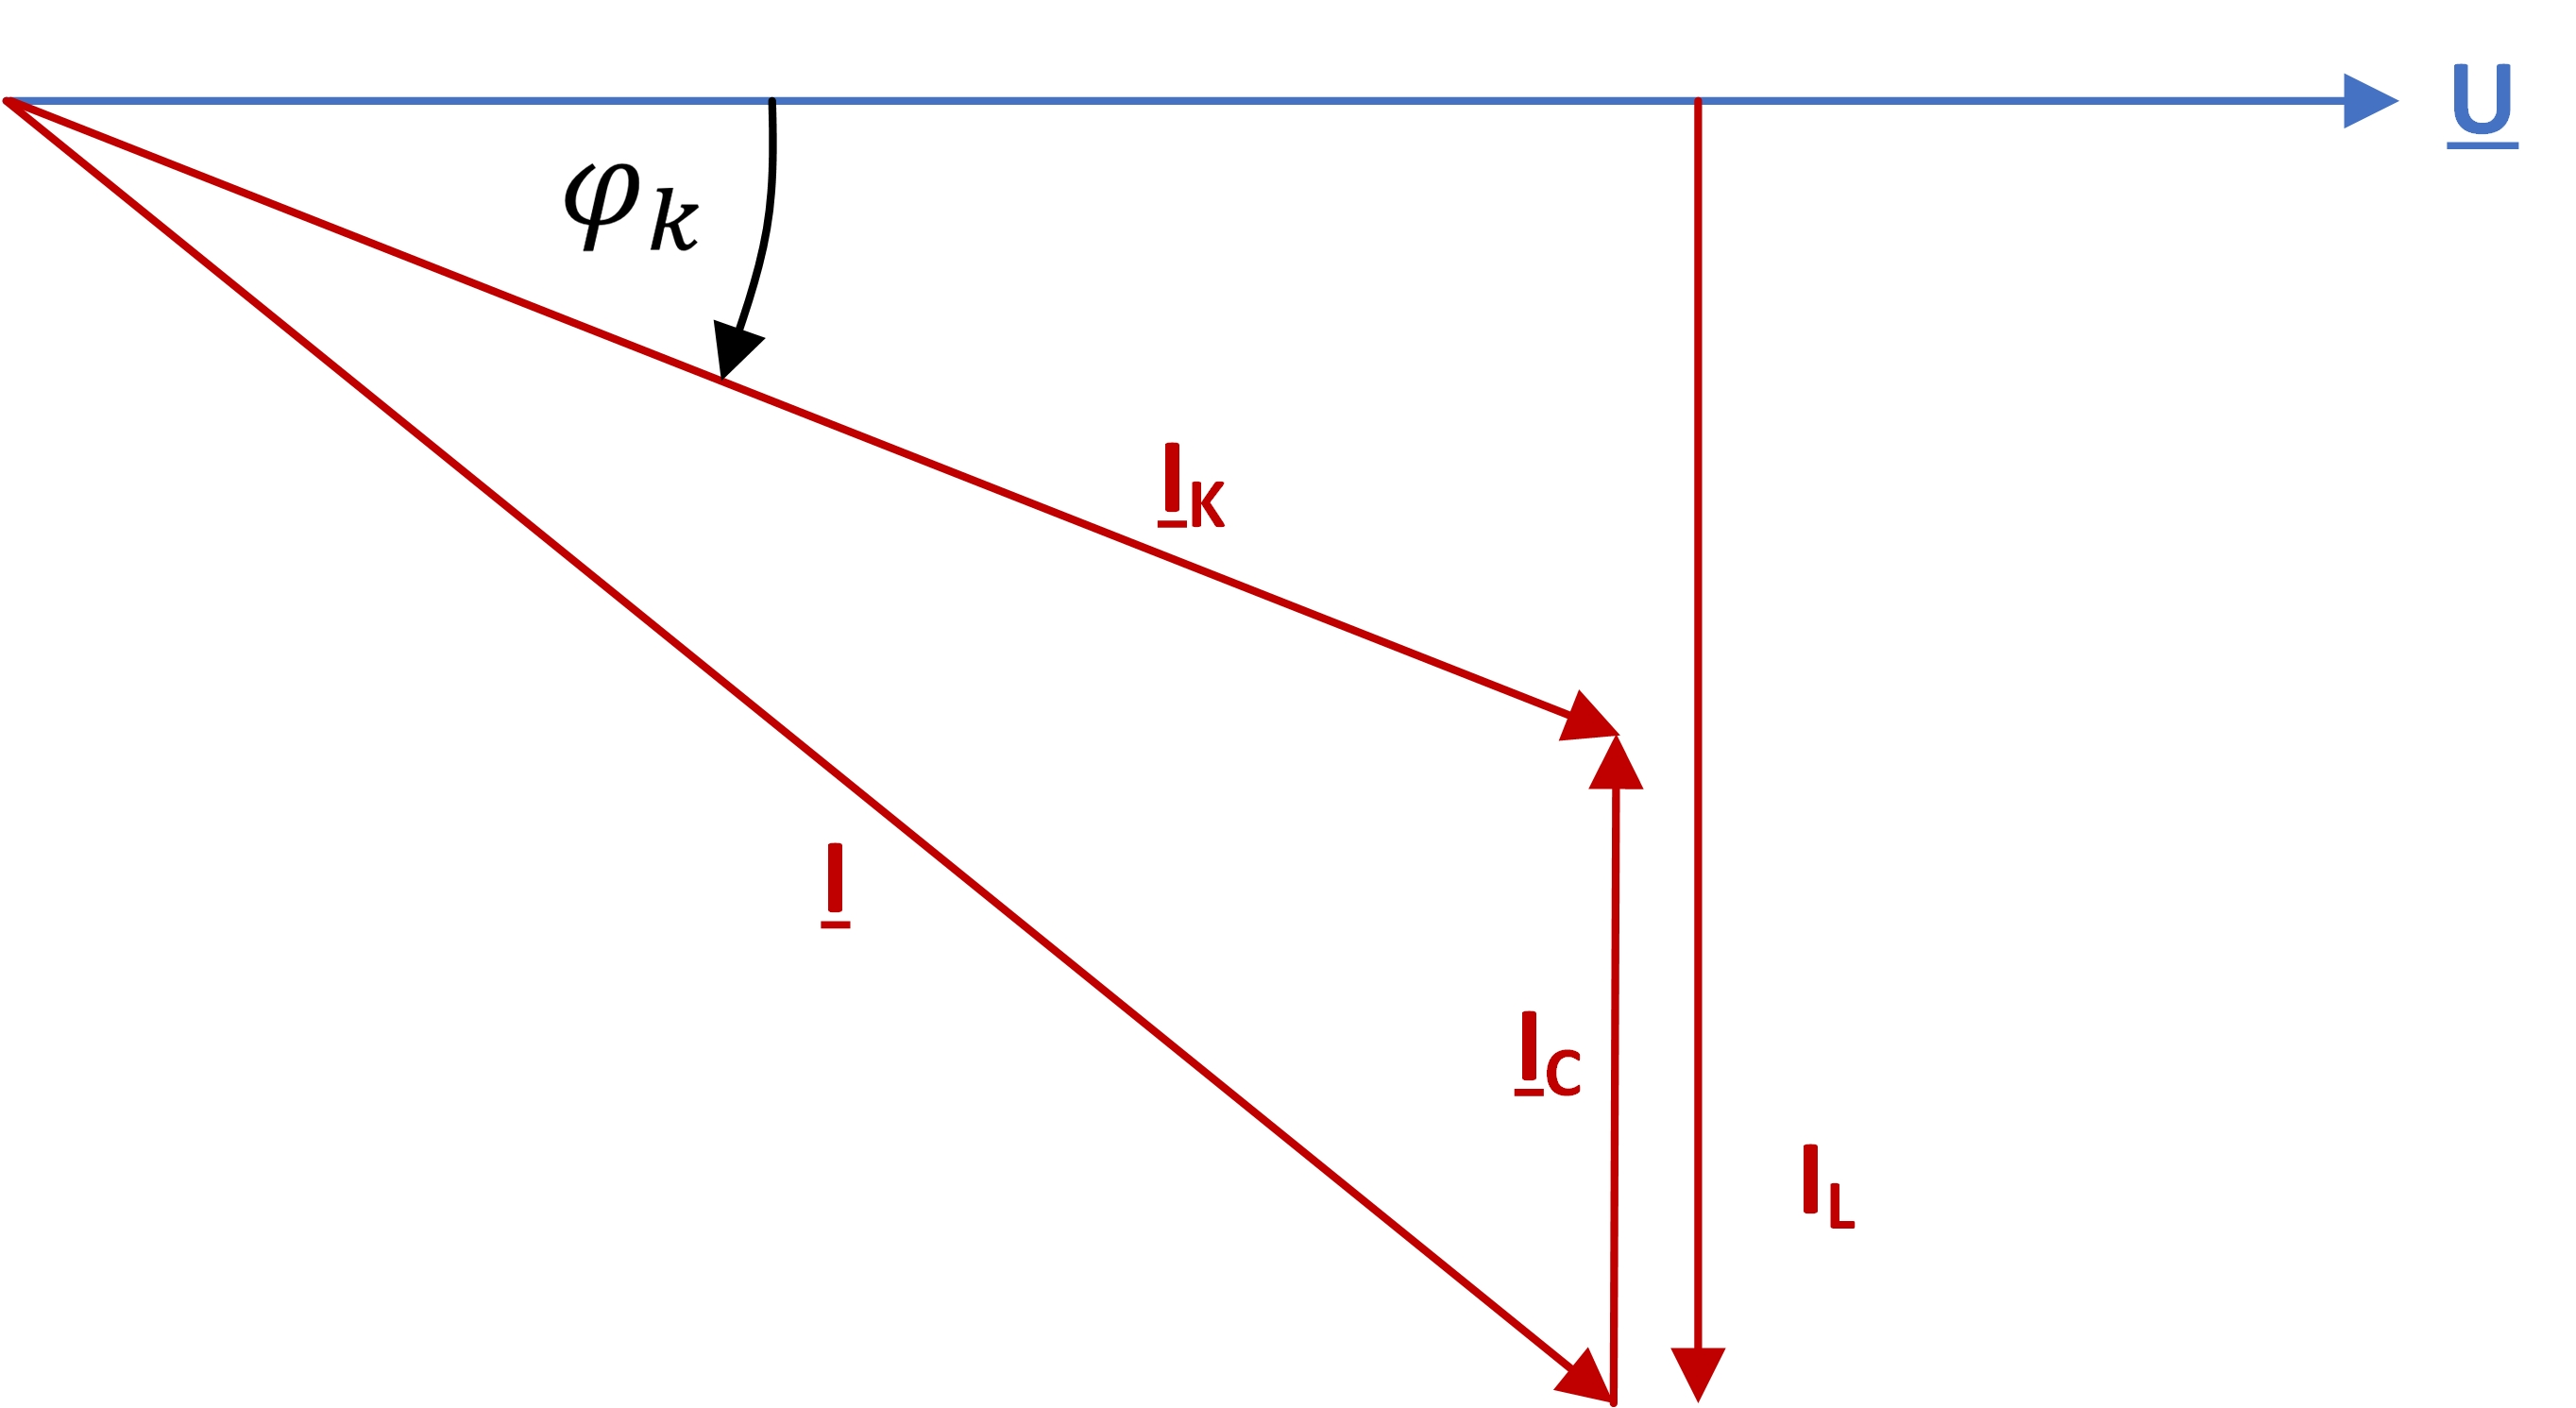
\includegraphics[width=3.5cm]{bilder/Parallel-Kompensation_RostBau.jpg} \newline
		\end{minipage} \\
	Blindwiderstände &
		\begin{minipage}{4.5cm}
			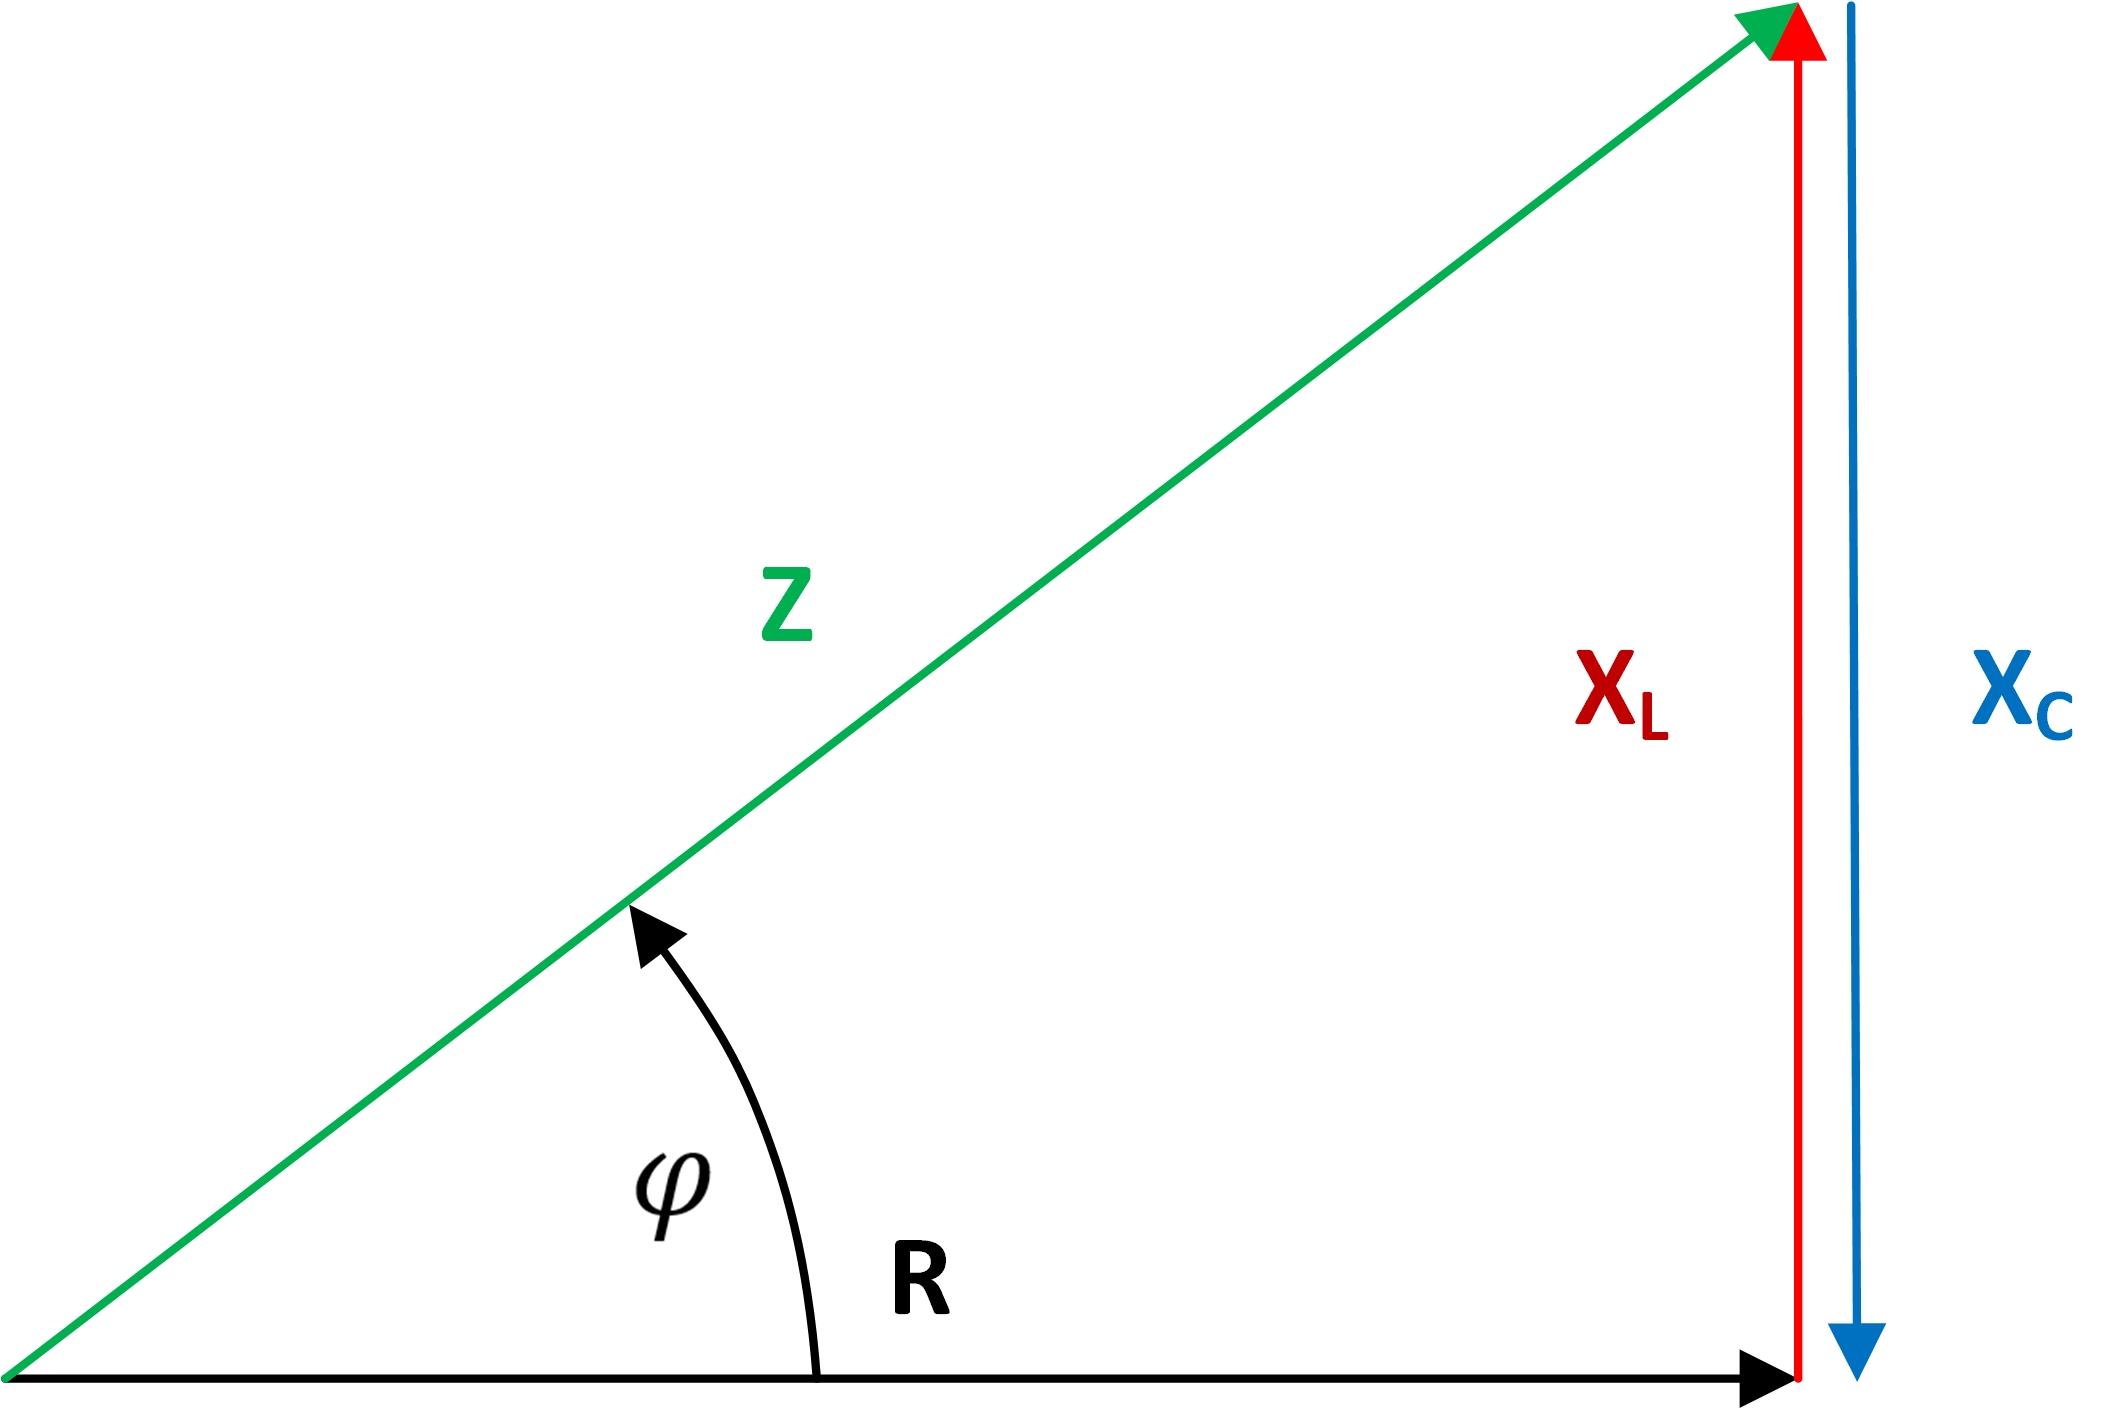
\includegraphics[width=3.5cm]{bilder/Seriell-Blindwiderstaende_RostBau.jpg}%%Blindstromkompensation.png%} \newline
		\end{minipage} &
		\begin{minipage}{4.5cm}
			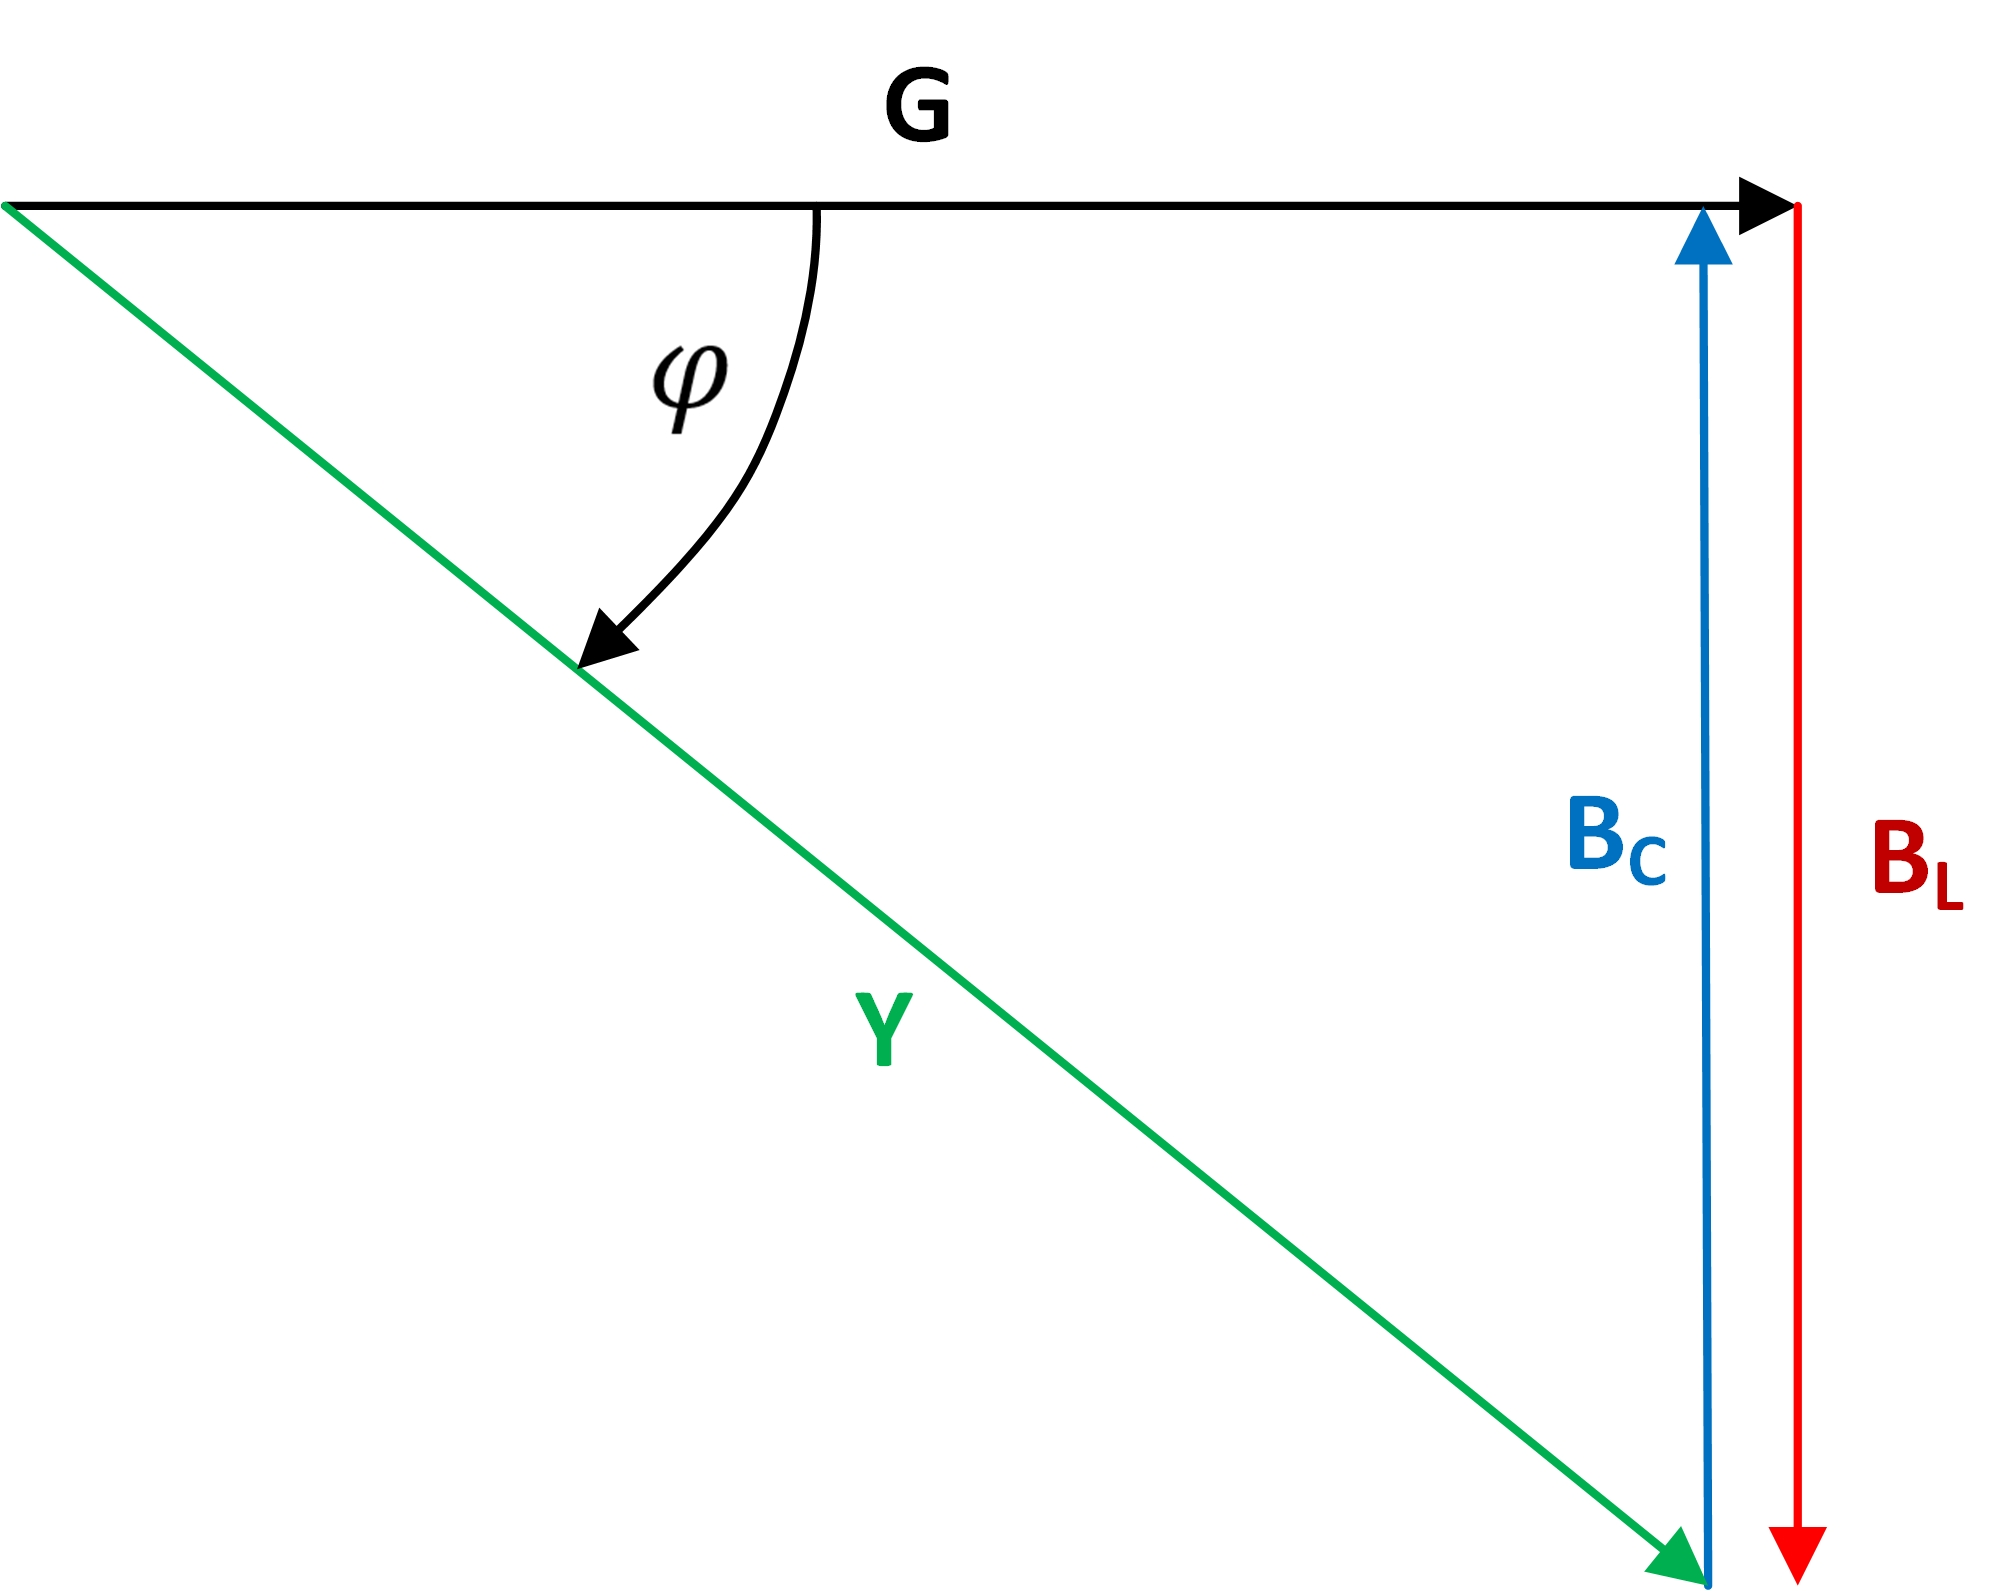
\includegraphics[width=3.5cm]{bilder/Parallel-Blindwiderstaende_RostBau.jpg} \newline
		\end{minipage} \\
	\hline
	Neue (kompensierte) Blindleistung &
		\multicolumn{2}{l}{$Q_{Lk} = P \cdot \tan{\varphi_k}$} \\
	Blindleistung des Kondensators & 
		\multicolumn{2}{l}{$Q_C = Q_{Lk} - Q_L =  P\cdot (\tan{\varphi_k}-\tan{\varphi}) $} \\
	Kapazität des Kondensators &
		\multicolumn{2}{l}{$C = - \frac{Q_C}{\omega U^2}$} \\
		\hline	
	\end{tabular}
\renewcommand{\arraystretch}{1}